This section contains all the use cases initially described with the use cases UML model, then the most important Use Case have their own table which provide further details such as: involved actors, entry conditions, flow of events,  exit conditions and exceptional conditions.

\subsubsection{User Page use cases}
\begin{figure}[htp] 

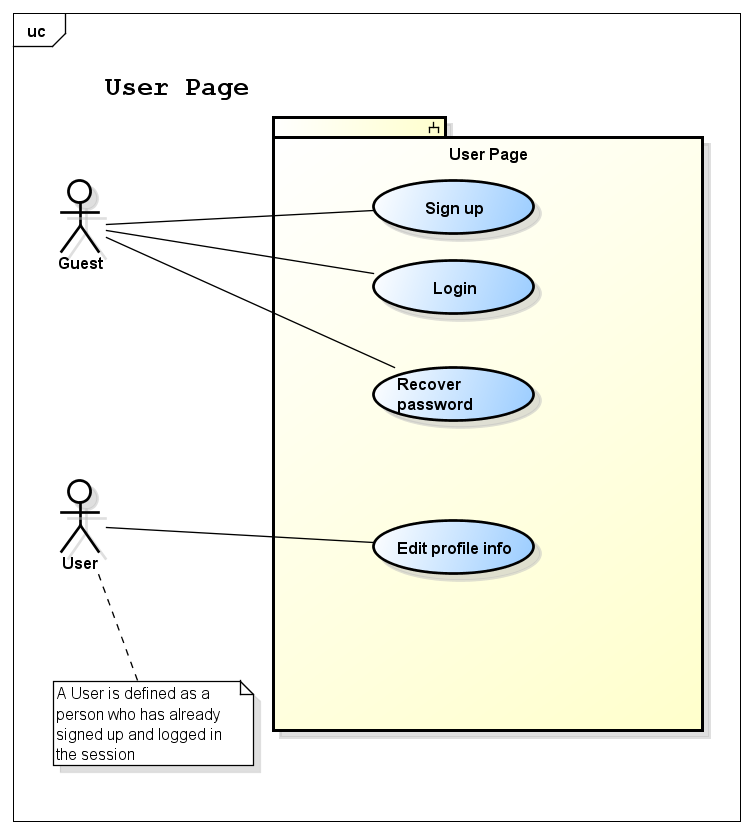
\includegraphics[width=\textwidth]{usecases/png/userpage} 
\caption{Use cases relative to the user registration and authentication} 
\label{fig:userpage} 
\end{figure} 

\newpage
\subsubsection{Sign up}

\begin{table}[htp]

\begin{tabular}{r|p{7cm}}
\bf\large Name&\bf\large Sign up\\
\hline
\hline
\bf Actors&Guest\\
\hline
\bf Entry conditions&None\\
\hline
\bf Flow of events&
\begin{itemize}
\item The guest reaches the registration page containing the relative form
\item The guest fills up the form and clicks on "Sign up" to complete the process
\item The system redirects the user to his profile page and sends a confirmation email.
\end{itemize}
\\
\hline
\bf Exit conditions&The guest has successfully registered in the system. \\
\hline
\bf Exceptions&The guest left an empty field or typed
 something wrong an error message is displayed 
 and the user is asked to fill the form again.\\
\hline

\end{tabular}
\caption{Sign up Use Case table} \label{tab:signup}
\end{table}


 \newpage
\subsubsection{Login}
\begin{table}[htp]

\begin{tabular}{r|p{7cm}}
\bf\large Name&\bf\large Login\\
\hline
\hline
\bf Actors&User\\
\hline
\bf Entry conditions&The user has already registered.\\
\hline
\bf Flow of events&
\begin{itemize}
\item The user reaches the login page containing the relative form
\item The user types the username and password in the login form and click on "Login" button.
\item The system redirects the user to the application homepage.
\end{itemize}
\\
\hline
\bf Exit conditions&The user has access to the application functionalities. \\
\hline
\bf Exceptions&Username and password didn't correspond or the username didn't exist ,an error message is displayed and the user is asked to fill the login form again.\\
\hline

\end{tabular}

\caption{This is my one big table } \label{tab:login}
%\autoref{fig:userpage}
\end{table}
\newpage
\subsubsection{Password Recovery}
\begin{table}[htp]
\begin{tabular}{r|p{7cm}}
\bf\large Name&\bf\large Recover Password \\
\hline
\hline
\bf Actors&User\\
\hline
\bf Entry conditions&The user has already registered.\\
\hline
\bf Flow of events&
\begin{itemize}
\item The user reaches the login page containing the relative form
\item The user clicks on "Password recovery" button and is redirected to the password recovery page.
\item The user inserts his email and clicks on "reset password".
\item The system sends an email to the user with a link and instruction to reset the password.
\item The user chooses and types a new password and confirms.
\item The system redirects the user to the login page.
\end{itemize}
\\
\hline
\bf Exit conditions&The user has changed his password \\
\hline
\bf Exceptions&The inserted email doesn't match any user in the database, it is displayed an error message and the user is asked to retype a valid email.\\
\hline

\end{tabular}
\caption{Recover password Use Case table} \label{tab:recoverpassword}
\end{table}


\newpage
\subsubsection{Schedule Management use cases}
\begin{figure}[htp] 
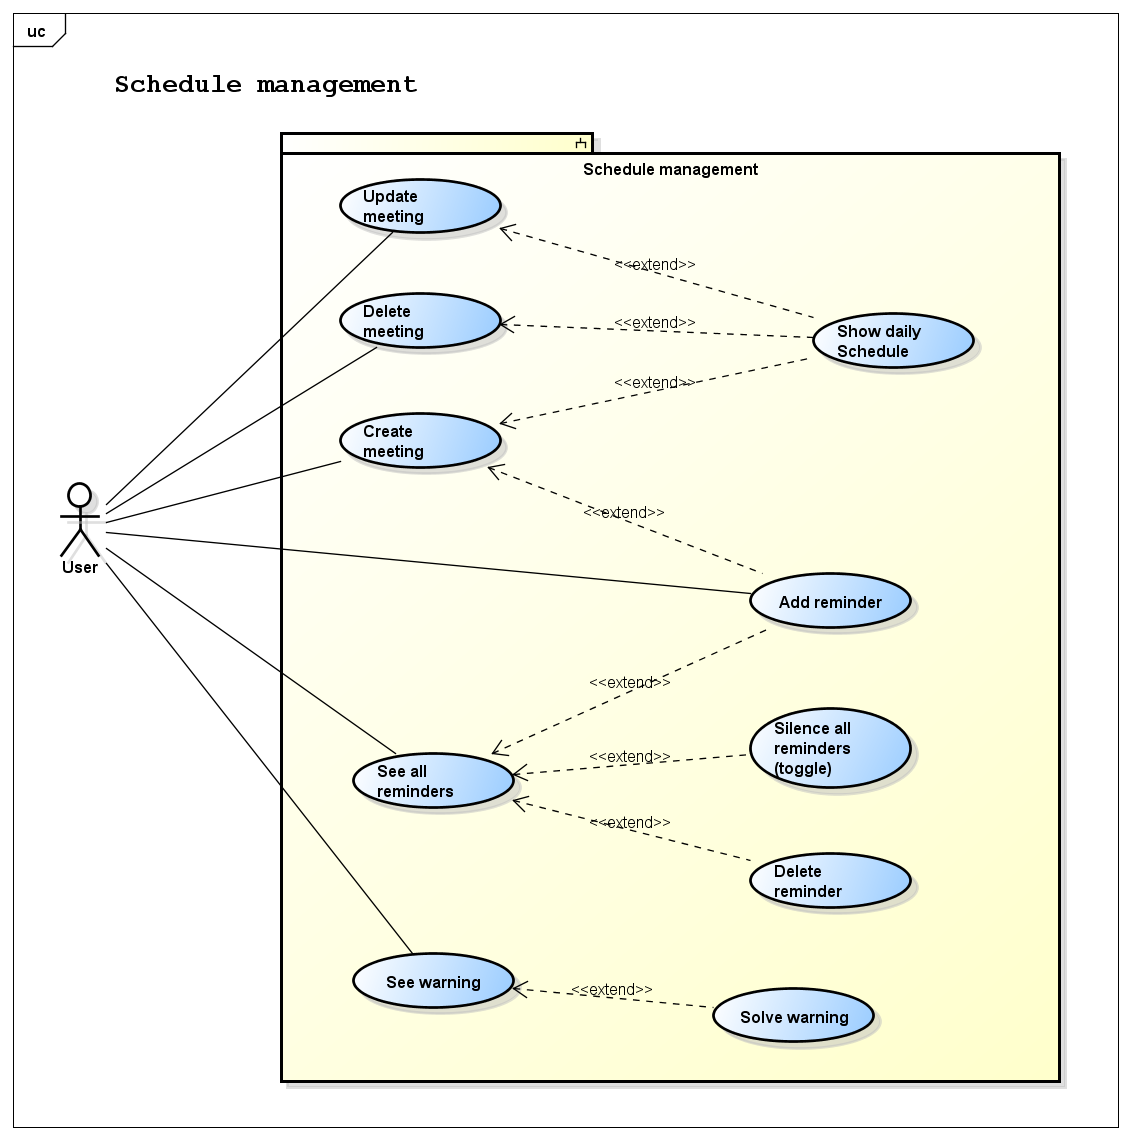
\includegraphics[width=\textwidth]{usecases/png/schedulemanagement} 
\caption{Main use cases showing the functionalities of Travlendar+ application relative to the meetings creation and management} 
\label{fig:schedulemanagement} 
\end{figure}

\newpage
\subsubsection{Meeting Creation}
\begin{table}[htp]

\begin{tabular}{r|p{7cm}}
\bf\large Name&\bf\large Creation of a meeting\\
\hline
\hline
\bf Actors&User\\
\hline
\bf Entry conditions&The user is logged in and is in the main page.\\
\hline
\bf Flow of events&
\begin{itemize}

\item The user clicks on "Create meeting" button and he is redirected to the page with the input form to create a meeting.

\item The user fills up the form with the meeting information (title, location, description, date and time, flags, etc...).

\item The system checks whether the meeting at the specified time and date is possible according to the user preferences and the current daily schedule, the optimal route is proposed.


\item The user is then redirected to the main page.

\end{itemize}
\\
\hline
\bf Exit conditions&The new meeting with the calculated optimal route is added to the user Calendar. In the case of the incompatibility of a meeting with others a warning is created.\\
\hline
\bf Exceptions&The information inserted is wrong or some information is missing: a corresponding error is displayed and the user is asked to modify the inserted information accordingly.
\\
\hline

\end{tabular}
\caption{Meeting Creation Use Case table}
 \label{tab:meetingcreationtab}
\end{table}
\newpage
\subsubsection{Meeting Deletion}
\begin{table}[htp]

\begin{tabular}{r|p{7cm}}
\bf\large Name&\bf\large Deletion of a Meeting\\
\hline
\hline
\bf Actors&User\\
\hline
\bf Entry conditions&The user is logged in and is in the page of a meeting\\
\hline
\bf Flow of events&
\begin{itemize}

\item The user clicks on "Delete meeting" button and he is asked by the system if he is sure he intends to perform that action.

\item If the user clicks "yes" then the meeting is deleted from the system.

\item The system checks if a Warning has to be calceled because of the meeting deletion and if it's the case it deletes the warning.


\item The user is then redirected to the main page.

\end{itemize}
\\
\hline
\bf Exit conditions&The meeting is not present in the system anymore, possibility of the cascade effect of a warning deletion.\\
\hline
\bf Exceptions&None
\\
\hline

\end{tabular}
\caption{Meeting Deletion Use Case table}
 \label{tab:meetingdeletion}
\end{table}
\newpage
\subsubsection{Reminder Addition}
\begin{center}
\begin{tabular}{r|p{7cm}}
\bf\large Name&\bf\large Addition of a reminder\\
\hline
\hline
\bf Actors&User\\
\hline
\bf Entry conditions&The user is logged in and is on the page of a meeting\\
\hline
\bf Flow of events&
\begin{itemize}
\item The user clicks on "Add reminder" button and he is redirected to the page with the input form to add a reminder.

\item The user fills up the form with the type of reminder and the time he wants to be reminded of the upcoming meeting.

\item  The system adds the reminder and the user is redirected to the relative meeting page.

\end{itemize}
\\
\hline
\bf Exit conditions&The reminder is added to the meeting \\
\hline
\bf Exceptions&There exists already an identical reminder and it is not added to the meeting\\
\hline

\end{tabular}
\end{center}
\newpage
\subsubsection{Warning Solving}
\begin{center}
\begin{tabular}{r|p{7cm}}
\bf\large Name&\bf\large Solving a warning\\
\hline
\hline
\bf Actors&User\\
\hline
\bf Entry conditions&The user is logged in and is in the page of a warning\\
\hline
\bf Flow of events&
\begin{itemize}
\item The user clicks on "Solve warning" button and he is redirected to a page that lets him
choose how to solve the conflict: the timing of two overlapping meetings can be changed, or one of the two meetings has to be canceled; 
\item  The user solves the conflict the way he wants and clicks on the button "Done".
\item  The system checks whether the conflict has been solved and the user is redirected to the warnings page.
\end{itemize}
\\
\hline
\bf Exit conditions&The warning has been solved and is deleted from the system and from the list of warnings in the corresponding page\\
\hline
\bf Exceptions&The warning was not solved after the user's modifications, the unresolved warning will still be present and a message stating that the conflict wasn't successfully solved is displayed. The user is redirected to the warning page.
\\
\hline

\end{tabular}
\end{center}


\newpage
\subsubsection{User Preferences use cases}
\begin{figure}[htp]
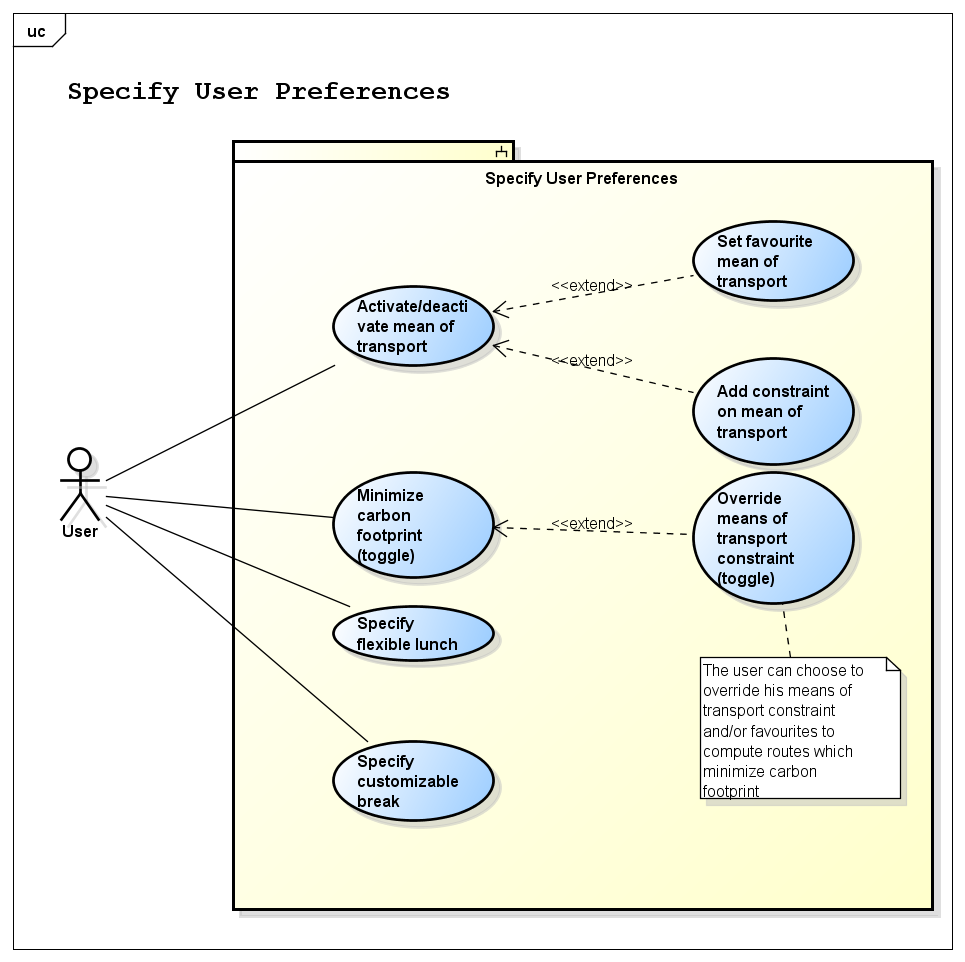
\includegraphics[width=\textwidth]{usecases/png/specifyuserpreferences} 
\caption{Use cases showing the user preferences and relative functonalities} 
\label{fig:specifyuserpreferences} 
\end{figure}

\newpage
\subsubsection{Means activation/deactivation}
\begin{table}
\begin{tabular}{r|p{7cm}}
\bf\large Name&\bf\large Activate/deactivate mean of transport\\
\hline
\hline
\bf Actors&User\\
\hline
\bf Entry conditions&The user is logged in and is in the user preferences page\\
\hline
\bf Flow of events&
\begin{itemize}
\item The user clicks on "Choose means of transport" button and he is redirected to a page containing a list of all possible means of transport;
\item  The user unflags all the means of transport he does not intend to use.
\item  The user clicks on "Done" button and is redirected to the user preferences page.
\end{itemize}
\\
\hline
\bf Exit conditions&The unflagged means of transport are removed from the possible means needed to compute a route\\
\hline
\bf Exceptions&The user unselected every mean of transport, clicking "Done" button has no effect and an error message stating that at lest one mean of trasport has to be flagged.
\\
\hline

\end{tabular}
\caption{This is my one big table} \label{tab:activatedeactivatemean}
\end{table}


